\chapter{Related Work}
\label{cha:relwork}

%\begin{itemize}
%\item Which similar/related works have been carried out?
%\item If applicable: structuring of related work is good (e.g., if you have multiple related fields)
%\item What is deficient in these works and what do they lack?
%\item Compare the existing approaches in a table (different approaches in rows, features/requirements in columns)
%and give a final discussion why a new approach (your thesis) is necessary
%\end{itemize}
There are three different types of complexities to handle big data systems \cite{p307}. These are:
\begin{itemize}
	\item Data complexity
	\item Computational complexity
	\item System Complexity
\end{itemize}
Data complexity arises due to the multiple formats \& unstructured of the data. Moreover data have huge number of dimensions and also there is a complexity between inter-dimensional and intra-dimensional relationships. The data complexity also increase the computational complexity in big data systems. Moreover,The extensive computational requirements of big data systems increase the system level complexity.\\\\
In the following two subsections we will describe the details of the past work of dimensionality reduction algorithm and Entropy Minimisation based reordering algorithm respectively.
\subsection{Related work with Dimensionality Reduction}
Efficient storage and retrieval of high-dimensional data certainly one of the major issue in database and data mining  research \cite{thesis2}. In the past, many attempts took to design multi dimensional indexing structure for example R-trees, $R^{*}$-trees, X-trees, SR-tree, etc. in order to speed up the query procedure. But these procedures fail to do so when the number of dimensions increases. The more is the number of dimension the more performance deteriorates. To overcome this issue, one way is to transform from high dimensional data to low dimensional data with the trade-off of limited information loss.\\\\
Though Dimensionality reduction is a very old problem but still this problem exists. Principle Component Analysis(PCA) and Linear Discriminant Analysis(LDA) are two mostly used one to reduce the number of dimensions. Both PCA and LDA seek directions of the component but the main difference among them is PCA seeks direction for representation where LDA seek directions for efficient discrimination. In both cases it assumes that training data set are available in advance but in reality a complete training set might not given beforehand.
\subsubsection{Principle Component Analysis}
PCA is a multivariate technique to analyze the data table. Here the observations are described by several inter-correlated quantitative dependent variables \cite{p314}. The goal is to find a subspace whose basis vectors correspond to the direction with maximal variances \cite{thesis1}. Mathematically, it depends on eigen decomposition by computing eigenvectors and eigenvalues and upon singular value decomposition (SVD) of rectangular matrices.\\\\
Lets denote $C = \frac{1}{n} \sum_{i=1,2,...,n}(x_i - m) (x_i - m)^T$ as the covariance matrix of the sample data. We define the objective function as \textit{J(W)} = \textit{trace$W^TCW$}. PCA aims to maximise the objective function \textit{J(W)} in a solution space \textit{$H^{d*p} = {W \in R^{d*P}, W^TW = I}$}.
\subsubsection{Linear Discriminant Analysis}
The goal of the Linear Discriminant Analysis (LDA) is used to find a lower dimensional space that best discriminants the samples from different classes \cite{thesis1}. In Linear Discriminant Analysis (LDA), we need to compute a linear transformation by maximising the ratio of the between-class distance to the within-class distance in target of achieving maximal discrimination \cite{p313}. After that we need to find eigen value decomposition of both matrix to select new feature subspace.
Mathematically the aim is to maximize the Fisher criterion an objective function: 
\begin{equation}
\textit{$ J(W) = \frac{W^TS_{b}W}{W^TS_{w}W} $} 
\end{equation}
where $S_{b} = \sum_{i=1}^{c}p_i(m_{i}-m) (m_{i}-m)^T$ and $S_w = \sum_{i=1}^{c}p_i \operatornamewithlimits{E}\limits_{x\in c_{i}} (x-m_{i})(x-m_{i})^{T}$ are called Interclass scatter matrix and Intraclass scatter matrix respectively. Here E denotes the expectation and $p_i = \frac{n_{i}}{n}$ is the prior probability of class i. We can get W by solving $W^{*}$ = arg max J(W) in the solution space $H^{d*p} = {W \in R^{d*p}, W^{T}W = I}$. This is done by solving the generalised eigenvalue decomposition problem: \textit{$S_{b}w = \lambda S_{w}w$}
\subsubsection{Limitation of PCA \& LDA}
By considering the availability of the data before applying algorithm is the main challenge in stream data application. In streaming data, data comes in a lot of numbers and continuous speed as a result it is not possible to store the data before applying algorithm. Moreover the traditional LDA and PCA perform in batch mode which is computationally expensive when dealing with large scale problems. In streaming data if there is a new data then both the LDA and PCA algorithm starts from the scratch to learn it from beginning which increase the computational complexity and large memory \cite{p316}.\\\\
Therefore, researchers look for the solution and one of the way to get rid of this to collect data whenever new data are presented and apply batch learning approach for the collected data so far. But the drawback of this approach is that it requires a large memory to store the data and high computational expenses are required. Moreover the system also forget about the knowledge that it acquires in past batch mode. Researchers work on this issue and some of their work are presented in the following section.\\\\
The another main challenge in streaming data is data may come into chunk from and also may be a single data in allowed form. That means the rate of data passing is unpredictable in nature therefore the dimensionality reduction algorithm should be adaptable with this issue.
\subsubsection{Principle Component Analysis for Streaming data}
Traditionally PCA efficiently represent high dimensional vectors with a small number of orthogonal basis vectors but this method is usually perform in batch-mode which is computationally expensive for large scale problems. To address this issue, researchers developed several incremental algorithms in their previous studies \cite{thesis4}.\\\\
Artac Jogan et. al \cite{p315} describes the way of remembering data from the sample and then delete the data to optimize the storage complexity. They used image as input where the representation of the image consists only of the corresponding coefficients stored as per image then the image is discarded. Here the performance is almost similar with the batch method but the learning method helps us to relearn data. Hall et.all \cite{thesis9}, Chandrasekaran et.all \cite{1thesis0}, DeGroat et.all also propose based on gaining information from the past and learn from the past and delete the data after acquiring the knowledge.\\\\
Li Xu et al. proposed an algorthm by removing the outliers. The estimation is done using the likelihood function.
All incremental PCA algorithm proposed so far is how to effectively handle with the covariance matrix but all of their effectiveness and computational complexity is more or less similar. Weng et all. \cite{thesis5} proposed a candid covariance free incremental analysis by using a well-known statistical concept efficient estimate like some well-known distribution for example Gaussian distribution. This algorithm also compute the principal component of samples incrementally without estimating the covariance matrix by keeping the scale of observations and computes the mean of observations incrementally. The main problem of this technique is to run into convergence problems in high dimensions.
\subsubsection{Linear Discriminant Analysis for Streaming data}
Similar to IPCA researchers also modify the LDA algorithm to run an incremental fashion to accomodate the new data. Here also one of the major concern is not forgetting prior knowledge.\\\\
Pang et. all \cite{1thesis2} propose the algorithm by adopting the system ready for any new data arrival in basis of single or chunk basis and termed separately sequential incremental LDA and chunk incremental LDA. In this paper they handle the eigenvectors by providing ranking and select the top most eigen vectors. This proposed algorithm will confront difficulty as the dimension if the data is very high. Specially it will require large memory hence it needs to solve a high dimensional generalised eigen value problem \cite{thesis3}.
Ye et.al \cite{thesis3} proposed an algorithm called Streaming LDA consisting three steps: first it compute the centroid matrix then update within-class scatter matrix. Finally the between-class scatter matrix is updated. After this steps, it also solve the eigenvalue problem.\\\\
kim et.all \cite{p317} propose a new concept to update between-class and within-class scatter matrix. They used sufficient spanning set to do so. In every step both matrices are kept and updated and minor components are removed in every step.\\\\
The main difficulty in all of the propose solution is the presence of the eigenvalue problem of scatter matrices which makes it difficult to maintain it incrementally. 
\subsubsection{QR decomposition}
LDA algorithm use Singular Value Decomposition(SVD). It is difficult to design an incremental solution for the eigenvalue problem on the product of scatter matrices.\\\\
To solve this, Ye Li et.al \cite{thesis2} propose an LDA based incremental dimension reduction algorithm called IDR/QR which applies QR decomposition rather than Singular Value Decomposition. The reason for using this technique is it does not require the whole data sets in memory before implementation. The algorithm is also computational cost efficient when new data item is inserted. The classification accuracy of this algorithm is very close in compare with the other best described LDA algorithm but it has much less cost when new items are inserted compare to others. Moreover hence it is computed some approximate matrices there is a chance of accumulating the approximate error as new data are appended sequentially. The larger the error the more the opportunity of information loss \cite{thesis3}.
\subsubsection{Fast Online incremental learning on mixture streaming data}
In \cite{p401} they proposed an algorithm for streaming data known as Fast Batch LDA algorithm known as FLDA/QR learning algorithm. In the algorithm they use the cluster centres to solve a lower triangular system which is optimized by the Cholesky-factorization. They also develop this algorithm for an exact incremental algorithm called IFLDA/QR. For reorthogonalization they use the Gram-Schmidt process which saves the space and time expense compared with the rank-one QR-updating of most existing methods. In there paper they mentioned their contributions are twofold:
\begin{itemize}
	\item They use the advantage of the QR-decomposition on a lower triangular matrix and propose a new fast batch method called FLDA/QR. In this algorithm, they take the centroid of each cluster to constitute the matrix decomposition. Because of this, they require a smaller storage and less computation. They also use the Cholesky-factorization which surpass in performance specially the computation load of the FLDA/QR method. 
	\item Next they develop an exact incremental version of the FLDA/QR known as the IFLDA/QR. It is mathematically possible to update the Gram-Schmidt reorthogonalization process. According to them, this process is faster than the rank-one updating in many other ILDA algorithms based on QR-decomposition.
\end{itemize}
The algorithm described in a paper is presented in the following figure \ref{fig:labelOfIFLDA} as a flow-chart.
\begin{figure}[htbp]
	% center the image.
	\centering
	
	% include a png file. Adapt size to 0.5 * textwidth and retain aspect ratio (!)
	\resizebox{\textwidth}{!}{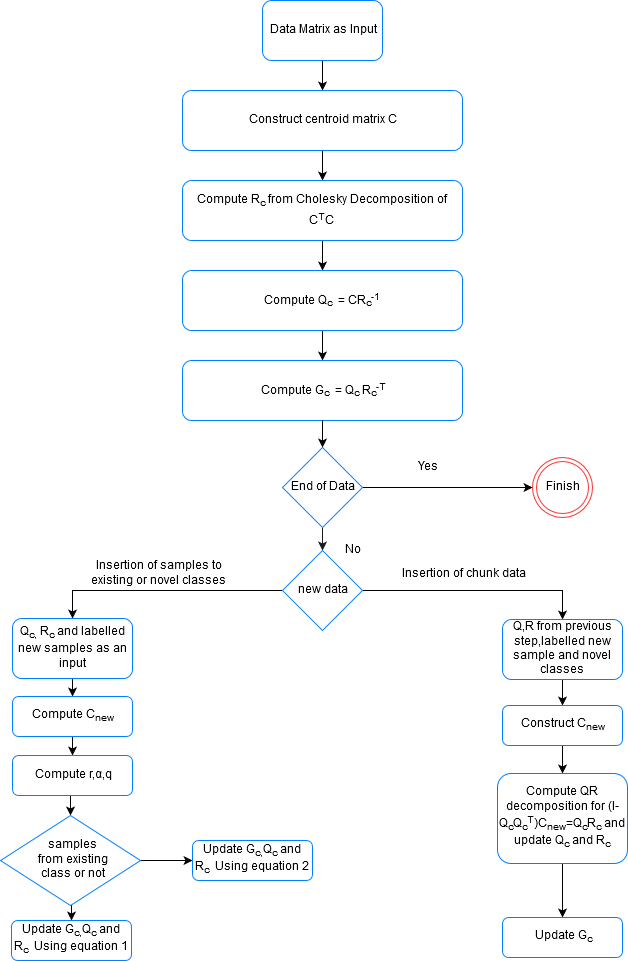
\includegraphics{IFLDA.png}}
	
	\caption{IFLDA/QR algorithm }
	\label{fig:labelOfIFLDA}
\end{figure}
The key characteristic of their algorithm which separates it from the other is the space and time complexity. It is space and time efficient compare to others while updating the algorithm because of the arrival of the data. This algorithm is 2 to 10 times faster than the state-of-the-art algorithm where the classification performance is same like the others.
\paragraph{Fast Batch Linear Discriminant Analysis:}
After having the data matrix as an input first the algorithm try to compute the global centroid matrix C consisting of the K centers. In this algorithm, lower triangular linear system is used for the calculation. Since the input training data is the centroid matrix therefore the scatter matrix within-class scatter is 0. They used the Cholesky-factorization to generate the matrix of R for the QR decomposiiton. The algorithm complexity is \textit{O(dn)}
\paragraph{Incremental Linear Discriminant Analysis:}
After development of the FLDA algorithm they extend the algorithm for the incremental development of the new incoming streaming data.The streaming data may come in three different forms:
\begin{enumerate}
	\item new labeled samples to the existing classes
	\item samples from an entirely new (novel) class
	\item a chunk of samples mixed with those as 1) and 2)
\end{enumerate}
In cases  1 \& 2, the samples from the existing classes and from an entirely new classes the updated calculation of the new centroid matrix is same. The r,$\alpha$,q is also calculated in the same way for both case. The difference lies within the update G\textsubscript{c}, Q$_c$ and R$_c$. The update version of any $variable$ is represented as $\hat{variable}$. If the the new labeled samples from the existing classes then the $Q_c$ \& $R_c$ are updated using equation \ref{existing class}  
\begin{equation} \label{existing class}
\hat{C} = Q_c*R_c
\end{equation}
For new novel classes data are updated by the equation \ref{existin_class_GC}
\begin{equation} \label{existin_class_GC}
\hat{G_c} =\begin{bmatrix}G_c -q{c_{new}}^T G_c/\alpha & q/\alpha\end{bmatrix}
\end{equation}
There may be a chunk of new data which contain samples from the existing classes and novel classes. The challenge in this case is to extract the information from these mixed data and also they need to preserve the previous learned ones. The current algorithms fail to perfom in this scenario. After constructing $C_{new}$ they compute the QR decomposition of $(I-Q_c{Q_c}^T)C_{new} = \hat{Q_c}\hat{R_c}$ and update $\hat{Q_c}$ and $\hat{R_c}$. Update the $\hat{G_c}$ using equation \ref{chunk_GC}
\begin{equation} \label{chunk_GC}
\hat{G_c} = \begin{bmatrix} G_c-\hat{Q_c}(\hat{R_c}^{-T}({C_{new}}^T)G_c) & 0\end{bmatrix} + \hat{Q_c}(\hat{R_c}^{-T}Z)
\end{equation}
\subsection{Related work with Entropy Minimisation Algorithm:}
Petrie introduced the model of how to order a data matrix in 1899. Later this is named as data reordering or seriation. This methodology is used in many different application disciplines for example archaeology, anthropology etc. Data ordering has huge impact on some cases for instance gene expression data analysis in bio-informatics, geographical data analysis, bandwidth minimization or data compression \cite{1thesis3}.\\\\
The main assumption of seriation in data visualization is based on the assumption of permuting either rows or columns of the dataset without loss of information. Therefore, data reordering is done in such a way that similar examples or features are close to each other. Closeness of data helps to improve the quality of visualization without loss of any information as data dimension reduction methods do.\\\\ 
The seriation of the dataset can be formalised as if there is a dataset having n objects \textit{O\textsubscript{1},...., O\textsubscript{j}} one can construct an n*n symmetric dissimilarity matrix \textit{D=(d\textsubscript{i,j})} where d\textsubscript{i,j} for $1 \leq $i,$j \leq $n represents the dissimilarity between objects \textit{O\textsubscript{i}} and \textit{O\textsubscript{j}}, and \textit{d\textsubscript{i,i} = 0} for all i. The major challenge in seriation problem is to find a permutation function.\\\\
Researchers proposed different permutation function for reordering data. Hahsler et al. \cite{p308} reviewed a larger number of permutation function such as column gradient measure, anti-robinson effects, Hamilton path length, inertia criterion, least squares criterion, linear seriation criterion, measure of effectiveness and stress measure.\\\\
To find the most loss/merit functions in discrete optimization problem is a complex problem. An exchaustive serach is infeasible because the number of possible permutations for n objects is n!. Researchers proposed different heuristics and seriation methods that are briefly covered in the following subsections.
\subsubsection{Entropy Minimization}
There are some loss functions used for data seriation which are related with entropy. For instance, in \cite{p309} author defined the stress measure as a sum of local entropy of each data item. To minimize the sum, Wilkinson proposed a heuristic approach \cite{p310} and Niermann proposed a genetic evolutionary algorithm \cite{p309}. The another way to encode the dataset using Differential Predictive Coding (DPC). In this method, each item is encoded as a difference between current and previous items. Djuric et al. proposed an efficient algorithm to minimize the entropy of the encoded dataset in \cite{1thesis3}.
\subsubsection{Travelling salesman problem solver}
Data reordering using the length of a Hamiltonian path as a loss function is equal to solving a Travelling Salesman Problem (TSP), which is a well known and extensively researched combinatorial optimization problem. The aim of an Travelling Salesman Problem Solver (TSP-solver) is to find the shortest tour that, starting from a specific city, visits each city exactly once and then returns to the starting point. As the general seriation problem, solving the TSP is also complex. In case of seriation with n + 1 cities, n! tours have to be checked. In order to avoid exhaustive search, different heuristics were proposed, from simple nearest neighbour methods to complex approaches like the Lin-Kernighan (LK) algorithm \cite{p308}. Recently, Djuric and Vucetic \cite{1thesis3} introduced a fast \textit{O(nlog2n)} TSP-solver, called the TSP-means.
\subsubsection{Hierarchical clustering}
Hierarchical clustering and its extension named Hierarchical clustering with optimal leaf ordering(HC-olo) are most commonly used methods in bioinformatics \cite{1thesis3}. The output of HC is a series of nested clustering which are stored in a tree. The order of leaf nodes in a tree is used to produce the linear order of the example. The problem is to find the optimal leaf ordering because a binary tree having n leafs and fixed tree structures have $2^{n-1}$ different linear orderings. To solve this issue, Bar-joseph et al. \cite{p311} proposed an optimization algorithm called HC-olo. The time complexity of \textit{O($n^3$)} is not at all suitable for big data.
\subsubsection{Low-dimensional projection algorithm}
Researchers also target to use the state-on-art dimensionality reduction algorithm for example, PCA, LLE, LDA to project the original dataset into one-dimensional subspace. The linear ordering of the examples is that new subspace can be used for reordering. The problem is the intention of any dimensional reduction method is not the reordering rather it is a byproduct of manifold search so the quality of produced ordering is not at all satisfactory.
\subsubsection{Sugiyama's algorithm}
To draw a bipartile graph with as few edge crossing as possible is a well-known NP-complete problem \cite{p312}. Sugiyama's algorithm is based on average heuristics approach for drawing problem. The backbone of the algorithm is to order nodes according to the average of their adjacent nodes in the opposite node set. To apply Sugiyama's algorithm for data reordering first Makinen et.al proposed first to make data into a binary format from the original dataset. Then we consider rows and columns of the matrix as two separate nodes sets, where binary values represent edges between nodes. In figure \ref{fig: Sugiyama's algorithm} shows applying the average heuristic to a simple bipartite graph.
\begin{figure}[htbp]
	% center the image.
	\centering
	
	% include a png file. Adapt size to 0.5 * textwidth and retain aspect ratio (!)
	\resizebox{\textwidth}{!}{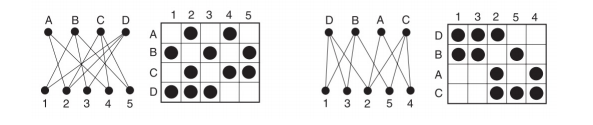
\includegraphics{Sugiyama_algorithm.png}}
	
	\caption{IFLDA/QR algorithm }
	\label{fig: Sugiyama's algorithm}
\end{figure}
\subsubsection{Entropy-Minimization-based data reordering}
In this section we will cover the algorithm that we will implement from data reordering representative. The algorithm will be presented shortly in this section. The approach that has been proposed in \cite{1thesis3} we will implement in the algorithm and modify it to adopt for data streaming. According to Djuric et.al \cite{1thesis3}:
\begin{itemize}
	\item Ordering can be done by doing permutation of rows or columns that ensures maximally compressible data set. The maximally can be determined by the entropy of the residuals of predictive coding.
	\item The problem is determined by an Expectation-Maximization algorithm which alternatively solves a TSP and assign reweights features based on the quality of the resulting tour.
	\item The proposed TSP solver known as TSP-means find the path comparable to those by LK algorithm. By applying K-means (k=2) recursively the algorithm construct a Binary tree. The runtime of TSP solver is \textit{O(nlog(n))}.
\end{itemize}

In next following paragraph we will describe the differential predictive coding, entropy minimisation reordering and TSP-means algorithm respectively.
\paragraph{Differential Predictive Coding:}
We assume our dataset D is stored in a form of n*m data table.
\[
\begin{bmatrix}
x_{11} & x_{12} & \dots & x_{1j} & \dots & x_{1m} \\
x_{21} & x_{22} & \dots & x_{2j} & \dots & x_{2m} \\
\vdots & \vdots & \ddots & \vdots & \ddots & \vdots \\
x_{i1} & x_{i2} & \dots & x_{ij} & \dots & x_{im} \\
\vdots & \vdots & \ddots & \vdots & \ddots & \vdots \\
x_{n1} & x_{n2} & \dots & x_{nj} & \dots & x_{nm}
\end{bmatrix}
\]
where i$^{th}$ row vector represent an example with m features.\\
Differential predictive coding replaces each example with its difference from the previous one, $\varepsilon_{i} = x_{i} - x_{i-1}$, where $\varepsilon_{i}$ is called DPC residual. As a result, the initial data table D is transformed into D\textsubscript{DPC} without loss of information since the original dataset can be retreived from the encoding.
\[
\begin{bmatrix}
x_{11} & x_{12} & \dots & x_{1j} & \dots & x_{1m} \\
\varepsilon_{21} & \varepsilon_{22} & \dots & x_{2j} & \dots & \varepsilon_{2m} \\
\vdots & \vdots & \ddots & \vdots & \ddots & \vdots \\
\varepsilon_{i1} & \varepsilon_{i2} & \dots & \varepsilon_{ij} & \dots & \varepsilon_{im} \\
\vdots & \vdots & \ddots & \vdots & \ddots & \vdots \\
\varepsilon_{n1} & \varepsilon_{n2} & \dots & \varepsilon_{nj} & \dots & \varepsilon_{nm}
\end{bmatrix}
\]
\paragraph{Entropy Minimization Reordering:}
In data compression theory entropy is used as a measure of randomness of the dataset, where the larger value of entropy denotes large randomness and small compression ratio. Small entropy denoted by $H_{DPC(\varepsilon)}$ means DPC residuals are small which implies D is a well ordered dataset. $H_{DPC(\varepsilon)}$ can be estimated as 
\begin{equation} \label{residuals}
H_{DPC}(\varepsilon) = - \frac{1}{n-1} \sum_{i=2}^{n} logP_\varepsilon(x_i-x_i-1)
\end{equation}
where $p_{\varepsilon} (\varepsilon)$ is the probability density of vectors $\varepsilon$.\\ 
The permutation of examples $\pi^*$ whose has minimize entropy of DPC residuals is the optimal one.
\begin{equation} \label{optimum_permutation}
\pi^* =\operatornamewithlimits{argmin}\limits_{{\pi}}(H^{\pi}_{DPC})
\end{equation}\\
Djuric et al. \cite{1thesis3} proposed a model $P_{\varepsilon}$ as Gaussian or Laplacian distribution that results in introduction of $\sigma = [\sigma_{1}\sigma_{2}...\sigma{m}]$- vector of m parameters. According to his paper equation 2 can be restated as:
\begin{equation}
(\pi^{*},\bar{\sigma}^{*}) = \operatornamewithlimits{argmin}\limits_{\pi^{*},\bar{\sigma}^{*}}(H^{\pi}_{DPC})
\end{equation}
For data reordering the reason for using expectation-maximization-like algorithm is used to find a permutation of examples $\pi$ which gives the minimize DPC residuals.\\\\
In M-step we need to find a permutation of examples $\pi$,which assumes $\sigma_j$ are known and find the entropy. This way is equivalent of solving TSP where features are downscaled using $\sigma_j$ and then TSP-means algorithm can be applied.\\\\
When the current ordering $\pi$ is found, the goal of E-step is to calculate new values of $\bar{\sigma}$ which in return minimizes $H^{\pi}_{DPC}$. We can derive the new parameters using following formula:
\begin{equation} \label{residuals}
\sigma_{j}^{2} = \frac{1}{n-1}\sum_{i=2}^{n}(x_{\pi(i),j}-x_{pi(i-1),j})^{2}
\end{equation}
\paragraph{TSP-means:}
To start TSP-means we need to recursively apply k-means clustering (k=2) to initial dataset to create binary tree T which follows a conversation from binary tree to $2^{l}$-ary tree $T^{l}$ by keeping only nodes at every $l^{th}$ tree level. After the conversation the algorithm traverse the tree in a breadth first way from left to right. The goal is to reorder internal and leaf nodes so that similar examples (leafs) and clusters (internal nodes) are closer to each other. To achieve this, we are going to use a TSP-solver for example: LK algorithm to reorder the children of the node together with their neighbours and replace the node by its reordered children.